\documentclass{beamer}

\mode<presentation>
{
  \usetheme{CambridgeUS}
  \setbeamercovered{transparent}
}

\usepackage[english]{babel}
\usepackage[latin1]{inputenc}
\usepackage{times}
\usepackage[T1]{fontenc} 
% Or whatever. Note that the encoding and the font should match. If T1
% does not look nice, try deleting the line with the fontenc.
\usepackage{amsmath}

\newcommand{\linespace}{\vskip 0.25cm}

\definecolor{MyForestGreen}{rgb}{0,0.7,0} 
\newcommand{\tableemph}[1]{{#1}}
\newcommand{\tablewin}[1]{\tableemph{#1}}
\newcommand{\tablemid}[1]{\tableemph{#1}}
\newcommand{\tablelose}[1]{\tableemph{#1}}

\definecolor{MyLightGray}{rgb}{0.6,0.6,0.6}
\newcommand{\tabletie}[1]{\color{MyLightGray} {#1}}

% The text in square brackets is the short version of your title and will be used in the
% header/footer depending on your theme.
\title[Mobile Security]{Improving Mobile Security}

% Sub-titles are optional - uncomment and edit the next line if you want one.
% \subtitle{Why does sub-tree crossover work?} 

% The text in square brackets is the short version of your name(s) and will be used in the
% header/footer depending on your theme.
\author[Luthi]{Braden Luthi}

% The text in square brackets is the short version of your institution and will be used in the
% header/footer depending on your theme.
\institute[U of Minn, Morris]
{
  Division of Science and Mathematics \\
  University of Minnesota, Morris \\
  Morris, Minnesota, USA
}

% The text in square brackets is the short version of the date if you need that.
\date[April '14, ] % (optional)
{29 April 2014 }

% Delete this, if you do not want the table of contents to pop up at
% the beginning of each subsection:
\AtBeginSection[]
{
  \begin{frame}<beamer>
    \frametitle{Outline}
    \tableofcontents[currentsection, hideothersubsections]
  \end{frame}
}

\begin{document}

\begin{frame}
  \titlepage
\end{frame}

% For a 20-25 minute senior seminar talk you probably want something like:
% - Two or three major sections (other than the summary).
% - At *most* three subsections per section.
% - Talk about 30s to 2min per frame. So there should probably be between
%   15 and 30 frames, all told.

\section*{Overview}


\subsection*{Outline}

\begin{frame}
  \frametitle{Outline}
  \tableofcontents[hideallsubsections]
\end{frame}
\section{Background}
\subsection{Cryptography}

	\begin{frame}
	\frametitle{Cryptography}
	
		Cryptography or 'secret writing' is the study and practice of techniques for securing communications between two parties. \linebreak
		\begin{itemize}
			\item \textbf{plain-text}  Readable message to be sent during communications.
			\item \textbf{cipher} method for transforming plain-text
	        \item \textbf{key} parameter for cryptographic algorithm		
			\item \textbf{cipher-text} Unreadable form of the message
			
		\end{itemize}		 
	%basic introduction to cryptography and vocabulary
	
	\end{frame}
	\begin{frame}
	\frametitle{Cryptography}
		\begin{itemize}
			\item \textbf{Symmetric cryptography} 
			Both parties share a secret key for encryption and decryption
			\item \textbf{Asymmetric cryptography}
			Each individual has a public and a private key. Parties use the public keys for encryption and the private keys for decryption
		\end{itemize}
	
	\end{frame}

\subsection{GSM and UMTS}
	\subsubsection{GSM}
		\begin{frame}
		\frametitle{GSM}
		Global System for Mobile Communications (GSM) is a 2G telecommunication standard developed in the early 90's by the European Telecommunications Institute. Has become one of the most widely used standards, reaching an 80\% market share at its height.
					
		\end{frame}
	\subsubsection{UMTS}
	\begin{frame}
		\frametitle{UMTS}
		Universal Telecommunications Standard (UMTS) is 3G telecommunication standard based on GSM by the Third Generation Partnership Project.   
	\end{frame}

	
\section{GSM Weakness in UMTS}

	

	\begin{frame}
	\frametitle{Encryption in GSM and UTMS}
	\begin{itemize}
	
	
		\item GSM and UMTS both have secret keys that are shared between the mobile and the mobile's home network authentication center.
		
		\item GSM and UMTS both utilize the A5 family of encryption algorithms. 
		 \begin{itemize}
			\item A5/0 
			\item A5/1
			\item A5/2
			\item A5/3 
		\end{itemize}
		\end{itemize}
		
	\end{frame}
	
\subsection{Authentication}
\begin{frame}
% add hidden frames, introduce requests one at a time
  \frametitle{GSM Authentication}
  \begin{center}
  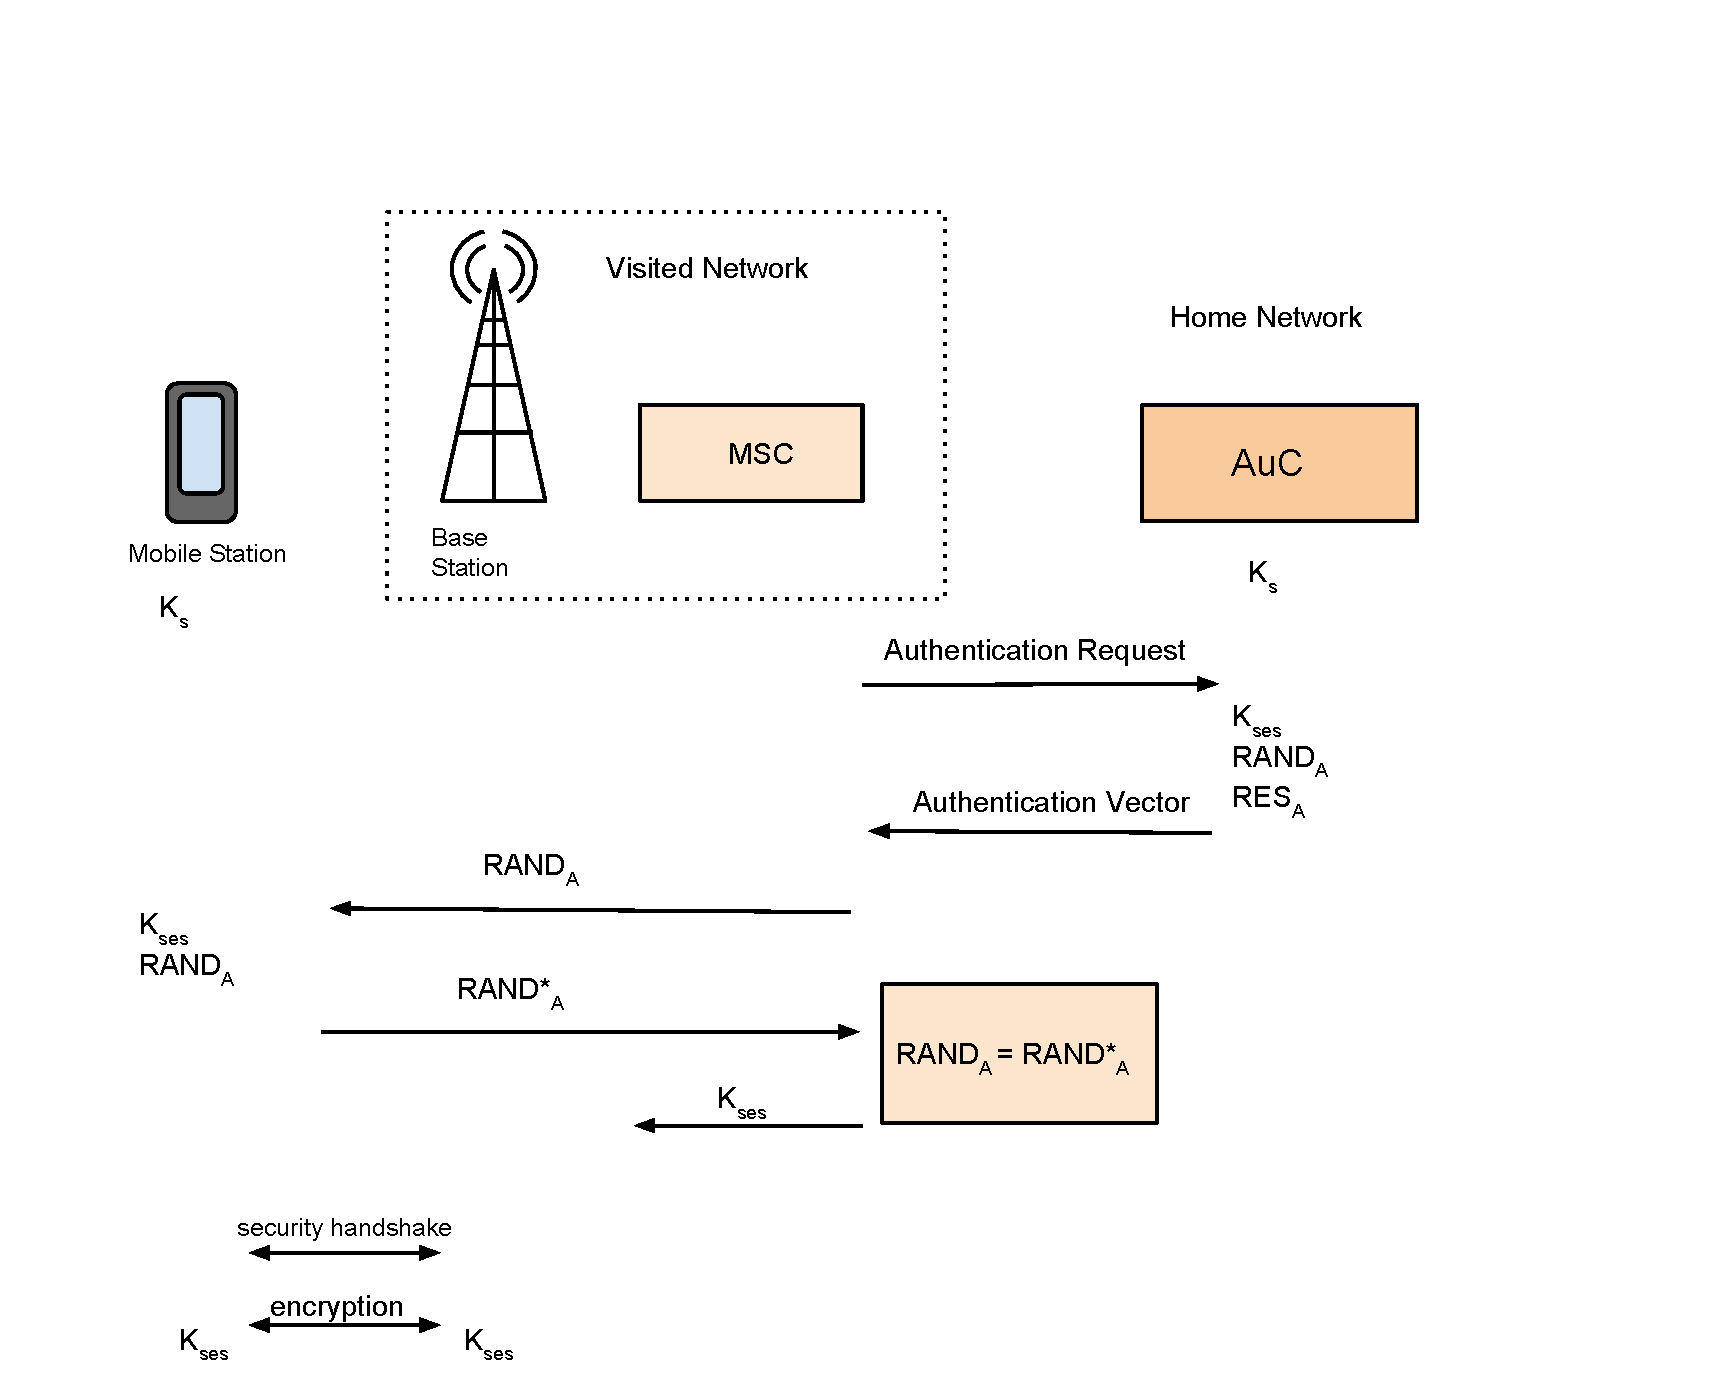
\includegraphics[scale =.32]{GSMAuthentication.pdf}

  \end{center} 
\end{frame}

\subsection{GSM and UMTS Inter-working Networks}
\begin{frame}
	\frametitle{Inter-working Networks}
\end{frame}
\subsection{Man-in-the-middle Attack}
\begin{frame}
		\frametitle{Man-in-the-middle Attack}
		% describe man in the middle attack
		\end{frame}
		
		% add man in the middle attack example		
		
		
\begin{frame}
	\frametitle{Man-in-the-middle weakness in GSM}
	% refer back to GSM authentication diagram ?
\end{frame}
\subsection{Solution}
\begin{frame}
\frametitle{Protecting UMTS from GSM Man-in-the-middle attack}
\end{frame}
\section{Application Security Threat}
	\subsection{Applications}
		\begin{frame}
		\frametitle{Applications (Apps)}
		\end{frame}
		\begin{frame}
		\frametitle{Application Permissions in Android}
		\end{frame}
		\begin{frame}
		\frametitle{Application Threat keyboard Key-logger}
		\end{frame}
	\subsection{Solution}
		\begin{frame}
		\frametitle{KBS Checker}
		\end{frame}
\section{EM Leaking Key Information}
	\subsection{Side channel attack}
		\begin{frame}
		\frametitle{What is a Side channel attack?}
		\end{frame}
		\begin{frame}
		\frametitle{RSA Example}
		\end{frame}
	\subsection{Side channel through EM }
		\begin{frame}
		\frametitle{Ranged Side channel}
		\end{frame}
		
		\begin{frame}
		\frametitle{Findings}
		\end{frame}
		
		\begin{frame}
		\frametitle{Solution}
		\end{frame}
\section{conclusion}
	\begin{frame}
		\frametitle{Conclusion}
		\end{frame}	
		
		\begin{frame}
		\frametitle{Questions}
			\begin{center}
			\Huge Questions?
			\end{center}
		\end{frame}	

\end{document}


